% options:
% thesis=B bachelor's thesis
% thesis=M master's thesis
% czech thesis in Czech language
% english thesis in English language
% hidelinks remove colour boxes around hyperlinks


% arara: xelatex: { shell: yes }
% arara: makeglossaries	
% arara: biber
% arara: xelatex: { shell: yes }
% arara: xelatex: { shell: yes }
\documentclass[thesis=B,czech,hidelinks]{../template/FITthesisXE}

\usepackage{ graphicx }		% graphics files inclusion
\usepackage{ dirtree } 		% directory tree visualisation
\usepackage{ longtable } 	% tables which Pandoc use
\usepackage{ lscape }		% to be able to rotate stuff
\usepackage{ metalogo }		% for \XeLaTeX
\usepackage{ multicol }		% for multiple columns

\bibliography{sources.bib}


% make list of acronyms
\makeglossaries
\newacronym{AJAX}{AJAX}{Asynchronous JavaScript and XML}
\newacronym{BI-DBS}{BI-DBS}{Databázové systémy}
\newacronym{BI-SI1}{BI-SI1}{Softwarové inženýrství I}
\newacronym{BI-SP1}{BI-SP1}{Softwarový týmový projekt 1}
\newacronym{BI-SP2}{BI-SP2}{Softwarový týmový projekt 2}
\newacronym{BP}{BP}{Bakalářská práce}
\newacronym{CI}{CI}{Continuous integration}
\newacronym{CMS}{CMS}{Content management system}
\newacronym{DBS}{DBS}{Databázové systémy}
\newacronym{DML}{DML}{Data manipulation language}
\newacronym{DP}{DP}{Diplomová práce}
\newacronym{FDD}{FDD}{Feature driven development}
\newacronym{FEL}{FEL}{Fakulta elektrotechnická}
\newacronym{FIT}{FIT}{Fakulta informačních technologií}
\newacronym{HTML}{HTML}{HyperText Markup Language}
\newacronym{KOS}{KOS}{Komponenta studium}
\newacronym{LS}{LS}{letní semestr}
\newacronym{MVP}{MVP}{Model-View-Presenter}
\newacronym{OBS}{OBS}{Organization Breakdown Structure}
\newacronym{PHP}{PHP}{PHP: Hypertext Preprocessor}
\newacronym{PMI}{PMI}{Project Management Institute}
\newacronym{RA}{RA}{Relational algebra / Relační algebra}
\newacronym{SP}{SP}{Softwarový projekt}
\newacronym{SQL}{SQL}{Structured query language}
\newacronym{TDD}{TDD}{Test driven development}
\newacronym{UI}{UI}{User interface}
\newacronym{UX}{UX}{User experience}
\newacronym{XML}{XML}{Extensible Markup Language}
\newacronym{XP}{XP}{Extrémní programování}
\newacronym{XSLT}{XSLT}{Extensible Stylesheet Language Transformations}
\newacronym{ZS}{ZS}{zimní semestr}
\newacronym{ČVUT}{ČVUT}{České vysoké učení technické}
\glsaddall	% add even unused acronyms

% % % % % % % % % % % % % % % % % % % % % % % % % % % % % % 

\acknowledgements{Na následujících řádcích bych chtěl poděkovat všem kolegům, kamarádům, mentorům i spolupracujícím studentům, se kterými jsem měl tu čest společně tvořit výukovou aplikaci, díky které mohla vznikout tato práce. Výčet bude dlouhý jelikož jsem u projektu již třetím rokem, a zejména studenti v realizačních týmech se střídají často. Nejprve musím samozřejmě poděkovat Ing. Jiřímu Hunkovi, který jakožto duševní autor aplikace, hlavní tester a vizionář nových požadavků a především jakožto vedoucí této práce, na toto místo patří. Dále musím zmínit dva excelentní studenty - Filipa Glazara a Pavla Kováře, kteří mi pomáhali s vedením týmů, podáváním zpětné vazby na kód studentů ale i řešením kritických chyb v produkční verzi, a to i přesto, že měli dost práce se svými vlastními bakalářskými pracemi. Zcela jistě patří díky i dalším výborným studentům, kteří pro DBS projekt vytvořili své bakalářské práce: Milanu Vlasákovi, Petru Pejšovi, Jiřímu Slavotínkovi, Martinu Kubišovi a Tomáši Fedorovi.\\
Při přesunu do historie musím každopádně uvést Jana Sýkoru, který mi především v začátcích, kdy jsem sám byl \emph{obyčejným studentem v předmětu BI-SP1}, radil, jak udělat mnoho věcí a naučil mne základ Gitu a Nette. Mezi další studenty, kterým bych chtěl poděkovat, lze každopádně zařadit všechny ty, kteří snáší pracovat pode mnou jakožto jejich projektovým manažerem - tedy studenty BI-SP1 a BI-SP2 napříč semestry od LS 2016 až po LS 2017. Jmenovitě se jedná o: Juraje Polačka, Milana Vancla, Vojtěcha Bakaje, Jakuba Nováka, Jakuba Štercla, Ladislava Zemka, Daniela Ondřeje, Lukáše Krčála, Ondřeje Lakomého, Richarda Strnada, Jana Luxemburka, Matěje Hlaváčka, Marka Erbena, Annu Dřevíkovskou, Davida Ryzce, Filipa Machalu, Jana Potočiara, Jakuba Dvořáka, Juraje Kožíka, Lukáše Banka a Marka Papinčáka.\\
Velké díky patří také Ing. Ivanu Halaškovi, za nahlašování obřího množství nedostatků a požadavků na funkcionalitu aplikace prostřednictvím veřejného bug reportu. Poděkovat bych také chtěl Ing. Michalu Valentovi a všem ostatním vyučujícím předmětu BI-DBS za snášení práce v portálu, který přes veškerou naši snahu stále obsahuje velké množství nedostatků.\\
Na závěr patří velké poděkování i Kristýně Miltnerové a Markétě Malcové za korekturu jazykové, gramatické a stylistické stránky této práce a mé rodině, za neutuchající podporu při mých studiích.}
\abstractCS{Práce se zaměřuje na efektivní řízení softwarového projektu, jehož cílem je vyvinout podpůrnou webovou aplikaci pro výuku předmětu BI-DBS na FIT ČVUT. Práce popisuje problémy s vedením vícečlenných týmů, zabývá se problematikou nasazování a udržitelnosti běhu výsledného softwaru a jeho průběžného vývoje. Cílem práce bylo navrhnout a začít používat postupy a nástroje, díky kterým se efektivně skloubí běžící systém a jeho průběžný vývoj za minimálního výskytu chyb. Jako metodika vývoje byla zvolena kombinace Extrémního programování a Feature-driven development, průběh práce je sledován v Redmine. Zdrojový kód aplikace je verzován a testován na Gitlabu. Poslední kapitola také obsahuje praktické ukázky konfigurace některých služeb potřebných pro běh samotné aplikace. Z práce lze vycházet při řízení jiných projektů obdobných rozměrů či pokračování v řízení stejného projektu.}
\abstractEN{This thesis focuses on effective software project management, which aims to develop a supporting application for teaching BI-DBS subject at FIT CTU. Thesis describes issues with leading a teams consisting of multiple people, deals with deployment, maintenance of deployed software and the development itself. The goal is to propose and start using procedures and tools, which will effectively combine a running system with its active development, while suppressing most of the bugs. The chosen software development methodology combines Extreme programming and Feature-driven development, the course of work is tracked in Redmine. Source code of the app is versioned and tested using Gitlab. The last chapter also includes samples of configuration for some services required to run the application. This work can be used as a base point for other projects with similar sizes or to continue in the process of managing the same project.}
\title {Řízení projektu a infrastruktury portálu pro podporu výuky předmětu BI-DBS}
\authorGN {Oldřich}
\authorFN {Malec}
\authorWithDegrees {Oldřich Malec}
\author {Oldřich Malec}
\supervisor {Ing. Jiří Hunka}
\keywordsCS {projektové řízení, metodiky vývoje, databázové systémy, řízení lidí, Redmine, Gitlab, SSL, Shibboleth, monitoring}
\keywordsEN {project management, development methodology, database systems, people management, Redmine, Gitlab, SSL, Shibboleth, monitoring}
\department {Katedra softwarového inženýrství}
\placeForDeclarationOfAuthenticity {V~Praze}
\declarationOfAuthenticityOption {4}
\website {https://gitlab.fit.cvut.cz/malecold/bc-thesis}
\assignment {../pdf/zadani.pdf}


\begin{document}

%\input{hyphenation.tex}

\begin{introduction} \label{introduction}
TODO úvod
TODO nějaká vlna
\end{introduction}

\chapter{Co je to DBS portál} \label{DBSportal}

Celá tato práce se zabývá vývojem a správou portálu pro předmět BI-DBS na FIT ČVUT. Ještě než se tedy ponoříme do jednotlivých součástí vývoje tohoto portálu, chtěl bych čtenáře seznámit s portálem samotným.

\section{Historie výuky BI-DBS}

Předmět Databázové systémy je vyučován na katedře softwarového inženýrství a v současném studijním programu se s ním setkají studenti první ročníku ve svém druhém semestru. Výkuka si klade za cíl přiblížit studentům problematiku ukládání dat, a to především pomocí relačních databází. Důraz je kladen na jazyky RA a SQL.

\paragraph{Semestrální práce}
Každý student si v rámci své semestrální práce vytvoří vlastní databázi, do které si poté vymýšlí dotazy za pomoci různých konstrukcí výše zmíněných jazyků. Typická semestrální práce obsahuje ve své fin8lní podobě alespoň 25 dotazů do databáze a pokrýva všechny standardní klauzule, které jazyk SQL nabízí.

\paragraph{Testy v semestru a zkouška}
Kromě semestrálních prací popsaných výše jsou také součástí hodnocení studentů průběžné testy v semestru a závěrečná zkouška. Testy v semestru se týkají především praktické části - tedy používání RA a SQL - které by student měl mít osvojené ze své semestrální práce. Závěrečná zkouška poté kromě praktických částí může obsahovat i teoretické otázky které byly probírány na přednášce či modelování schémat databáze.

\section{Vznik DBS portálu} \label{DBSportal:creation}
Obě výše popsané součásti výuku jsou poměrně náročné na korekturu vyučujícím. Typicky nebylo možné zajistit, aby vyučující zkontrolovatl každý jednotlivý dotaz, který student vytvořil ve své semestrální práci. Oprava testů, které se psali na papír poté trvala zbytečně dlouho a prakticky nebylo možné ji automatizovat. Z tohoto důvodu přišel v roce 2013 Jiří Hunka - jeden z vyučujících předmětu BI-DBS - s nápadem, že se realizuje portál zaměřený na podporu výuky Databázových systémů, který bude umožňovat jak efektivnější korekturu studentských semestrálních prací, tak rychlejší opravu testů a zkoušek.

\paragraph{Řešitelský tým}
Vývoj portálu takových rozměrů však nebylo možné financovat běžně dostupnými prostředky, kterými fakulta disponuje. Z toho důvodu bylo rozhodnuto, že bude portál vyvíjen s rámci předmětů BI-SP1 a BI-SP2. Jedná se o předměty vyučované také v oboru Softwarové inženýrství, které si studenti typicky zapisují ve svém 4., respektive 5. semestru studia. Cílem předmětů je vytvořit 3-5 členné týmy, které budou pracovat na softwarovém projektu, počínaje návrhem, analýzou požadavků atp. a konče hotovým softwarem. Bylo tak vypsáno zadání na realizaci DBS portálu, do kterého se přihlásilo 13 studentů.
Tento způsob záskávání pracovní síly pro další vývoj portálu je používán dodnes. Jelikož SP1 a navazující SP2 má celkové trvání jeden akademický rok, jsou každý rok nabíráni noví studenti. Toto přináší jak obtíže s řízením projektu, tak příležitosti pro jeho změny. Řízení DBS projektu se věnuje kapitola \ref{DBSmanagement}.

\paragraph{Nasazení portálu}
Portál byl poprvé nasazen do výuky v LS 2016, kdy byl využíván pouze na cvičeních, která vedl Jiří Hunka a ve zkouškovém období byl otestován také na jednom termínu závěrečné zkoušky.
V ZS 2016 portál používali všichni studenti, kteří měli předmět BI-DBS zapsaný, protože jich v tomto semestru bylo pouze 36, a jednalo se tak o ideální testovací vzorek pro příští semestr. Následující semestr - LS 2017 - již byl portál využíván i ostatními cvičícími mimo Jiřího Hunku a počet studentů se pohyboval kolem 550. Detailům ohledně nasazování portálu se věnuje kapitola \ref{infrastructure}

\chapter{Metody řízení projektu} \label{methods}

V druhé kapitole bych se chtěl věnovat především tématu metodik vývoje softwaru. Cílem je krátce čtenáře seznámit se standardními a agilními metodami vývoje softwaru a zaměřit se na možnosti jejich aplikace pro vývoj DBS portálu, který byl popisován v kapitole \ref{DBSportal}

\section{Tradiční metody} \label{methods:traditional}

\subsection{Vodopádový model} \label{methods:waterfall}

Jak zmiňuje \cite{kadlec}, nejedná se přímo o metodiku, ale pouze o životní cyklus. Je charakteristický tím, že všechny fáze vývoje jsou prováděny postupně za sebou a není možné se vracet. Případné změny je možní zpracovat až v rámci údržby, která vývoj vždy vrátí do jedné z předchozích etap a následně musí proběhnout i etapy následující.
Tento model vznikl již v roce 1970 a dnes se tedy dá považovat za zastaralý. Pro vývoj DBS portálu je tedy zcela jistě nevhodný.

\subsection{Spirálový model} \label{methods:spiral}

Vzniku Spirálového modelu dala za vznik především kritika Vodopádového modelu. Hlavní novinkou zde byl \emph{iterativní přístup} a opakovaná \emph{analýza rizik}. V tomto modelu se stále opakují fáze \emph{Stanovení cílů}, \emph{Analýza rizik}, \emph{Vývoj a testování} a \emph{Plánování}. Při každém průchodu těmito fázemi se provádí odlišná činnost než v předchozí iteraci (kromě analýzy rizik, ta je prováděna vždy stejně), například fáze vývoje v první iteraci pracuje pouze s koncepty, v příští iteraci specifikuje požadavky, v další navrhuje architekturu a teprve poté implementuje a testuje.\\
Stále se však jedná převážně o jednosměrnou cestu, která nejen na počátku ale i v průběhu obsahuje velké množství analýz a návrhů. Pro potřeby vývoje DBS portálu, kde se každý rok mění složení studentů, je tedy nevhodný.

TODO more std methods?

\section{Agilní metody} \label{methods:agile}

Agilní metody řízení vznikly především z důvodu neustále se měnících požadavků na software a rychlejší reakci na požadované změny. Tradiční metody nebyly schopné reagovat na změny požadavků dostatečně rychle. Především když se začneme bavit o vývoji softwaru, kde se neustále mění dostupné technologie a požadavky na finální verzi, jsou tradiční metody zcela nevhodným modelem vývoje.

Rozdíl mezi tradiční a agilní metodikou lze popsat také jejich přístupem k \emph{Funkcionalitě}, \emph{Času} a \emph{Zdrojům} \cite{kadlec}. Zatímco u tradičních metod je funkcionalita stanovena na začátku a musí být dosažena pomocí \emph{nějakého} času a \emph{nějakého} množství zdrojů, u agilních metod je to přesně naopak. Typicky je stanoven termín a dostupné zdroje a funkcionalita \emph{nějaká} bude.

Připomeňme si také \emph{Manifesto for Agile Software Development}\cite{manifesto}, který vznikl v roce 2001:

\begin{quote}
Objevujeme lepší způsoby vývoje software tím,
že jej tvoříme a pomáháme při jeho tvorbě ostatním.
Při této práci jsme dospěli k těmto hodnotám:
\begin{itemize}
	\item \emph{Jednotlivci a interakce} před procesy a nástroji
	\item \emph{Fungující software} před vyčerpávající dokumentací
	\item \emph{Spolupráce se zákazníkem} před vyjednáváním o smlouvě
	\item \emph{Reagování na změny} před dodržováním plánu
\end{itemize}
Jakkoliv jsou body napravo hodnotné,
bodů nalevo si ceníme více.

© 2001, výše zmínění autoři
Toto prohlášení může být volně kopírováno v jakékoli formě,
ale pouze v plném rozsahu včetně této poznámky. 

TODO change the last par - smaller font, grey color...

\end{quote}

Je tedy zřejmé, že Agilní metodiky více pracují s vývojáři samotnými, a umožňuji i potlačení některých postupů pro dobro celkua dovolují "zanedbat" i náležitosti jako třeba dokumentaci. Následně se na některé agilní metodiky zaměříme více:

\subsection{Extrémní programování}

XP rozvíjí standardní postupy, avšak posouvá je až do extrémů.
\begin{itemize}
	\item Vždy budeme pracovat na co nejjednodušší verzi, která splňuje požadavky
	\item Pokud se osvědčuje \emph{revize kódu}, budeme neustále revidovat kód \ldots
	\item Pokus se odvědčil \emph{návrh}, budeme neustále navrhovat a vylepšovat specifikaci \ldots
	\item Pokud se osvědčilo \emph{testování}, budeme neustále testovat \ldots
\end{itemize}
TODO rozvést, proč ne pro DBS...

\subsection{Scrum}

\chapter{Řízení DBS projektu} \label{DBSmanagement}

Kapitola popisuje řízení DBS projektu, jeho předešlý stav, návrhy na vylepšení a zhodnocení aplikovaných řešení. Zabývá se především efektivností řízení lidských zdrojů, komunikace a použitých technologií.

\section{Řízení lidských zdrojů}

Projekt je vývíjen již od roku 2014 v rámci předmětů BI-SP1 a navazujícího BI-SP2. Někteří studenti po dokončení BI-SP2 pokračují v práci na systému v rámci své bakalářské práce. Výjimečně jsou také vypsány samostatné bakalářské či diplomové práce zaměřující se na specifickou komponentu systému.
Ze studentů předmětů BI-SP1, případně BI-SP2 jsou typycky sestaveny 2-3 týmy po 4-5 členech.
TODO vedoucí týmu atp.

\section{Řízení komunikace}

Hlavním stěžejním bodem komunikace byla vždy pravidelná týdenní schůzka, na které se sešly řešitelské týmy s vedoucím práce - Ing. Jiřím Hunkou. Kromě těchto schůzek byl pro komunikaci využíván systém projektového řízení Redmine (popsáno v \ref{infrastructure:redmine}). Další komunikace nebyla jednotně stanovena a probíhala tak v různých komunikačních kanálech.
TODO rozvoj, Slack...

\subsection{Zpětná vazba}

Zpětná vazba probíhá standardně ze strany vedení projektu. Před realizací této práce tak byla veškerá zpětná vazba realizována především na pravidelných týdenních schůzkách, příležitostě také v systému probjektového řízení - Redmine.
Týmy také měly stanoveny své vedoucí, kteří řídili tým interně. Vedoucí týmu na schůzce prezentuje výstupy jeho týmu a popisuje, co který člen realizoval. Týmy se samy interně hodnotí v několika iteracích rozložených do celého semestru.
TODO rozvoj, bodování

\section{Nástroje}

Pro jakékoliv řízení projektu je potřeba využívat určitých nástrojů. Správě infrastruktury v projektovém řízení je v této práci věnována samostatná kapitola \ref{ch:infrastructure}.

\chapter{Infrastruktura DBS projektu} \label{infrastructure}

Z předchozích kapitol již víme, jak efektivně vyvíjet software a jak řídit lidské zdroje. V poslední kapitole své práce bych se chtěl věnovat infrastruktuře - tedy softwaru, procesům a nástrojům, které při vývoji DBS portálu využíváme.\\
V této kapitole často zmiňuji práci \emph{manažera projektu}, čímž mám na mysli svou vlastní práci.

%%%%%%%%%%%%%%%%%%%%%%%%%%%%%%
%%%%%%%%%%%%%%%%%%%%%%%%%%%%%%
%%%%%%%%%%%%%%%%%%%%%%%%%%%%%%

\section{Issue tracker}

Základním stavebním kamenem jakéhokoliv projektu, je \emph{issue tracker}, neboli \uv{systém sledování úkolů}. Do něj jsou zadávány úkoly, které je potřeba realizovat. Tyto úkoly se poté přiřazují lidem, kteří je budou řešit, a všechny změny úkolu jsou vždy jednoduše dohledatelné a měřitelné. Do těchto systémů je také často možné zaznamenávat čas strávený řešením daného úkolu, nastavovat termíny, hierarchie úkolů a řídit přístup různých rolí k určitým funkcionalitám.\\
Při vývoji DBS portálu využíváme následující issue trackery:
\begin{itemize}
	\item \emph{Redmine:} interní issue tracker využívaný vývojovým týmem a manažerem. Přístup k němu mají pouze role definované v předchozí kapitole v organizačním členění vývoje projektu (Obrázek \ref{picture:obs}). Slouží pro vývoj, rozdělení práce i záznam času.
	\item \emph{Gitlab:} veřejný issue tracker dostupný všem studentům i vyučujícím na FIT ČVUT, který slouží jako \emph{bug report} neboli \uv{hlášení chyb}. Chyby zde nahlašují typicky koncoví uživatelé portálu a z vývojového týmu na ně reaguje pouze manažer projektu, který poté potřebné úkoly zadává na interní issue tracker: Redmine.
\end{itemize}

\subsection{Redmine} \label{if:redmine}

\begin{quote}
\quotedblbase Redmine je flexibilní webová aplikace pro správu řízení projektu. Díky použití frameworku Ruby on Rails je multiplatformní a multidatabázová\textquotedblleft \cite{redmine}.
\end{quote}

Redmine je při vývoji DBS portálu využíván především pro:
\begin{itemize}
	\item Shromažďování úkolů k řešení.
	\item Sledování práce na přiřazeném úkolu.
	\item Záznam času stráveného řešením úkolu či u projektu.
	\item Shromažďování návodů a dokumentací - Wiki.
\end{itemize}
Jednotlivé body si následně popíšeme blíže, předtím bych však ještě chtěl zmínit možnost rozdělení úkolů do jednotlivých \emph{projektů}.

\subsubsection{Projekty v Redmine} \label{if:redmine:projects}

Redmine umožňuje na jedné instalaci provozovat několik oddělených (a nebo hiararchicky uspořádaných) projektů. V rukou hlavního administrátora (kterého u DBS projektu zastávám také já) je možnost umožnit určitým uživatelům či rolím přístup k různým projektům a také udělit různé pravomoce v těchto projektech.\\
Pro vývoj DBS portálu využíváme následující projekty:
\begin{itemize}
	\item \code{newDBS}: projekt shromažďující veškeré úkoly, které bude potřeba řešit, nemají však zatím přiřazeného řešitele.
	\item \code{SP-DBS-2017}: projekt zastřešující projekty jednotlivých týmů studentů, kteří mají zapsané předměty BI-SP1/BI-SP2. Tento projekt a jeho dílčí subprojekty se obměňují každým rokem, podle aktuálního počtu přihlášených studentů. V letním semestru 2017 se tento projekt dále dělí na:
	\begin{itemize}
		\item \code{Team 1}
		\item \code{Team 2}
	\end{itemize}
\end{itemize}

\paragraph{Proč dělit práci na projekty?}
Rozdělení na projekty je v běžné firmě jasné. V jednu chvíli se může pracovat na projektech několika klientů, které se sebou vůbec nemusí souviset. Proč ale dělit práci na projekty i u DBS portálu, který je jako celek pouze jeden projekt? Důvodem je především možnost využívání hromadných statistik, ale také rozdělení na realizační týmy.\\
Rozdělení má význam ve chvíli, kdy chce vedoucí týmu nebo manažer projektu zobrazit například celkový strávený čas jednoho z týmů, nebo zobrazení přidělené práce danému týmu. Díky odlišným projektům je snadné rozdělit úkoly, na kterých pracuje Team 1, Team 2 a nebo které nejsou zatím přiděleny k realizaci. Také vedoucí týmů mají snazší práci s přehledem práce svého vlastního týmu, mohou si zapnout emailové notifikace pouze pro změny v projektu, který patří jejich týmu atp.

\subsubsection{Shromažďování úkolů k řešení}

Během práce na projektu často vyvstávají nové požadavky či se objevují nové chyby. Tyto chyby a požadavky je potřeba \emph{ihned} zaznamenávat do issue trackeru. K tomu slouží projekt \code{newDBS}, který slouží jako \uv{shromaždiště úkolů}, které jsou \emph{volné} k řešení.\\
Odtud úkol typicky putuje dále zásahem manažera, který rozhodne o nutnosti jeho realizace a přiřadí úkol do jednoho z týmů - tedy projektu \code{Team 1} nebo \code{Team 2}. Některé úkoly jsou řešeny i přímo zde, ale to pouze výjimečně - na těch pracuji buďto přímo já nebo některý ze studentů pracujících na BP či DP.\\
Úkol, který je nově vytvořen v \code{newDBS} projektu má typicky vyplněna pouze následující pole:
\begin{itemize}
	\item \emph{Název:} stručný název úkolu. Na začátku názvu mohou být dodatečné popisné \emph{tagy}, například \code{[databaze]} nebo \code{[menu]}, které jasně definují, které komponenty systému se úkol týká.
	\item \emph{Popis:} detailní zadání úkolu, obsahující kroky k replikaci chyby, popis požadavku či nástin, jak úkol řešit.
	\item \emph{Stav:} výčet stavů, v tuto chvíli nastaven na \emph{Nový}. Všechny změny stavů popisuje \nameref{picture:activity} dostupný v příloze \ref{picture:activity}.
	\item \emph{Priorita:} priorita úkolu, u většiny úkolů nastavena na \emph{Normální}. Dalšími možnými stavy je \emph{Nizká}, \emph{Vysoká}, \emph{Urgentní} a \emph{Okamžitá}.
\end{itemize}


\begin{figure}[H]
\includegraphics[width=\textwidth]{../png/redmine.png}
\caption{Prostředí zadávání nového úkolu do Redmine} \label{picture:redmine}
\end{figure}

\subsubsection{Sledování práce na přiřazeném úkolu}

Jakmile je úkol přeřazen do jednoho z týmů, vyplní manažer i další dostupná pole:
\begin{itemize}
	\item \emph{Přiřazeno:} pole, které určuje člověka, po kterém je k úkolu požadován další vstup. Proces změny tohoto pole také popisuje \nameref{picture:activity} dostupný v příloze \ref{picture:activity}.
	\item \emph{Uzavřít do:} úkolu se nastaví termín, do kterého musí být vyřešen. V případě nevyřešení může být tým, kterému byl úkol přiřazen, bodově penalizován.
	\item \emph{Body:} manažer odhadne obtížnost řešení úkolu a přiřadí mu určité bodové ohodnocení. Více o bodování bylo probíráno v sekci \ref{ppl:ranking}: \nameref{ppl:ranking}.
\end{itemize}

V tuto chvíli přechází úkol do kompetence daného týmu, který na úkolu začne pracovat a postupně vykazuje svůj postup. K tomu slouží jednak možnost přidávat k úkolu komentáře, jednak možnost měnit pole \emph{\% Hotovo} a také zaznamenávat strávený čas (viz sekce \ref{redmine:time}).

Průběh práce je také možné sledovat na \emph{gitu}, respektive \emph{Gitlabu}, kterým se více věnují samostatné sekce \ref{version:git}, respektive \ref{version:gitlab}.

\paragraph{Návaznost commitů v gitu na Redmine úkoly} \label{redmine:commitlink}
Redmine umožňuje k projektu připojit i repozitář - v našem případě git. Při takovém provázání je vhodné, aby jednotlivé commity v gitu byly určitým způsobem provázány s úkolem, který řeší. Toho lze docílit přidáním ID úkolu do \emph{commit message}. Jedná se o jedno z pravidel pro psaní commitů, kterým se blíže věnuje sekce \ref{version:git:commit}. Takto provázané commity se poté zobrazují pod úkolem vedle poznámek uživatelů a je možné si je jednoduše otevřít a zobrazit změny v kódu.

\paragraph{Automatický report chyb v testech} \label{redmine:CI_report}
Jelikož nové \emph{commity} jsou po nahrání do sdíleného repozitáře testovány automatickými testy, je možné ihned zjistit případné nedostatky řešení. Pokud se při automatickém testu objeví chyba, je přes Redmine API přidán komentář k úkolu, ke kterému se commit váže, s informací, že test selhal, a s odkazem na Gitlab.

\paragraph{Provázání commitů na Gitlab}
Kromě automatického reportu chyb, který zrealizoval Pavel Kovář v rámci své BP, jsem také já upravil zdrojové kódy naší instalace Redmine pro snazší integraci Redmine a Gitlab. Jak již bylo zmíněno výše, Redmine sám zobrazuje u úkolu příslušné commity, samotné zobrazení commitu ale nedosahuje takových kvalit jako dedikované řešení: Gitlab. Z toho důvodu jsem k zobrazení odkazu na commit přidal i odkaz na Gitlab, jak znázorňuje obrázek \ref{picture:redmineTOgitlab}.
\begin{figure}[h]
\includegraphics[width=8cm]{../png/redmineTOgitlab.png}
\caption{Stav před a po nasazení úpravy kódu Redmine pro zobrazování odkazu na Gitlab} \label{picture:redmineTOgitlab}
\end{figure}

\paragraph{Dokončení úkolu}

Když je úkol dokončen, je dle workflow (příloha \ref{picture:activity}) přiřazen zpět na manažera, který zhodnotí kvalitu výstupu a vyplní pole \emph{Získané body}. Množství získaných bodů se odvíjí od předem stanovené bodové dotace za daný úkol a kvality jeho řešení definované v tabulce \ref{table:ranking}. 

\subsubsection{Záznam času} \label{redmine:time}

Řešitel úkolu si k němu také zaznamenává strávený čas, spolu s poznámkami, na čem v zaznamenané době pracoval. Tento čas se poté zobrazuje u úkolu a lze tak sledovat, zda byl odhad doby řešení správný, nebo je potřeba zvýšit časovou či bodovou dotaci. Také je možné v přehledu projektu či projektů zobrazovat, kolik hodin kteří uživatelé odpracovali a podle toho například rozdělovat hodnocení jejich práce.\\
Je však nutno zmínit, že záznam času není vždy ideálním měřidlem výkonu uživatele. Stejně obtížný úkol může zkušený programátor zrealizovat během 20 minut, kdežto nezkušený nováček může nad úkolem strávit i několik hodin a výstup i přesto zůstává sporný. Pro hodnocení by tak kromě vykázaného času měl být brán ohled i na kvalitu výstupu, případně další ukazatele.

\subsubsection{Wiki}

Redmine poskytuje také možnost tvorby \emph{knowledge base} či \emph{Wiki}, kterou využíváme především u newDBS\footnote{Dle rozdělení projektů v Redmine v sekci \ref{if:redmine:projects}} projektu. Informace zde shromažďované slouží jak pro podporu nových studentů, tak jako dokumentace aplikace. Jsou zde návody jak nasadit vývojové prostředí, spouštět testy, požadované formáty kódu i commit message a další. Struktura Wiki v současnosti vypadá následovně:
\begin{itemize}
	\item Instalujeme projekt - \emph{Sekce popisující nasazení vývojové verze projektu na počítač programátora}
	\begin{itemize}
		\item Vagrant
		\begin{itemize}
			\item Instalace a používání
			\item Integrace do PHPStorm
			\item Debug Selenium testů
			\item Řešení problémů
		\end{itemize}
		\item Manuální instalace
	\end{itemize}
	\item První spuštění a konfigurace nástrojů - \emph{Popis prvotního nastavení aplikace a vývojových nástrojů}
	\begin{itemize}
		\item První spuštění aplikace
		\item Kontrola code style
		\item Integrace s Tracy v PHPStorm
		\item Integrace Codeception s PHPStorm
	\end{itemize}
	\item Code practices - \emph{Seznam pravidel pro vývoj projektu. Obsahuje informace jako například požadavky na formátování a strukturu kódu, pojmenovávání tabulek databáze, strukturu commit message v gitu a další}
	\item Testování - \emph{Informace o tvorbě a spouštění automatických testů aplikace}
	\begin{itemize}
		\item Základní informace
		\item Tvorba testů
		\item Správa CI
	\end{itemize}
	\item Issue tracker, hodnocení - \emph{Informace o používání redmine}
	\begin{itemize}
		\item Redmine workflow - \emph{\nameref{picture:activity}, který je v této práci dostupný v příloze \ref{picture:activity}}
		\item Veřejný issue tracker na GitLabu
		\item Bodové hodnocení - \emph{Popis bodového hodnocení, v této práci popsaného v sekci \ref{ppl:ranking}}
	\end{itemize}
	\item Technologie - \emph{Dokumentace používaných technologií}
	\begin{itemize}
		\item Nástroje a task runner
		\item Databázové migrace
		\item Dokumentace různých komponent systému
	\end{itemize}
	\item Repozitář - \emph{Informace o repozitáři, návod jak používat git}
	\begin{itemize}
		\item Gitlab
		\item Doporučený git workflow
	\end{itemize}
	\item Server - \emph{Informace o serveru, na kterém výsledná aplikace běží}
	\begin{itemize}
		\item Datadog monitoring - \emph{Informace o Datadogu, v této práci blíže popsáno v sekci \ref{app:datadog}}
		\item Offsite zálohy - \emph{Informace o zálohách nahrávaných na externí úložiště}
	\end{itemize}
\end{itemize}

Je tedy jasné, že v případě jakýchkoliv nejasností je Wiki výchozím místem, kde hledat informace o projektu a všem, co s ním souvisí. Podoba Wiki se v průběhu času mění, jelikož nejen aplikace samotná, ale i způsob jejího vývoje prochází inovacemi.\\
Je důležité na Wiki zaznamenávat i dokumentaci různých procesů, které většina členů projektu využívá pouze uživatelsky a nikoliv administrativně, a to především z důvodu, aby byl \emph{kdokoliv v projektu nahraditelný}. Kvalitní dokumentace umožní při výpadku člena týmu pokračování ve vývoji i v případech, kdy se daný člen staral například o nasazování aplikace na server nebo spravoval jinou důležitou součást.

\subsection{Gitlab}

Gitlab je druhým issue trackerem využívaným při vývoji DBS portálu. Používá se pro \emph{spojení s koncovými uživateli}, kteří zde nahlašují chyby. Jelikož issue tracker na Gitlabu je jednodušší než ten na Redmine a všichni studenti i vyučující na FIT ČVUT jsou na něm automaticky registrováni, je vhodný pro využití právě veřejného bug reportu.\\
Já jakožto manažer projektu jsem emailem upozorňován na všechny nově nahlášené bugy či žádosti o podporu s používáním aplikace a snažím se na úkoly v co nejkratší době reagovat. Podpora uživatelů je typicky vyřízena do několika hodin, opravy chyb či požadavky nových funkcí jsou však interně předány na Redmine a poté zadány k realizaci týmům studentů, z toho důvodu může jejich vyhotovení trvat dny až týdny.\\
Uživatelé aplikace se k tomuto issue trackeru dostanou přes proklik přímo z aplikace, je však dostupný i přes link \url{https://gitlab.fit.cvut.cz/malecold/newDBS-bug/issues}.
\begin{figure}[h]
\includegraphics[width=\textwidth]{../png/gitlab-bug.png}
\caption{Nahlášené úkoly veřejného bug reportu v Gitlabu} \label{picture:gitlab-bug}
\end{figure}

%%%%%%%%%%%%%%%%%%%%%%%%%%%%%%
%%%%%%%%%%%%%%%%%%%%%%%%%%%%%%
%%%%%%%%%%%%%%%%%%%%%%%%%%%%%%

\section{Verzování a testování}

Prakticky jakýkoliv projekt, na kterém pracuje více lidí nebo trvá více než několik hodin je potřeba \emph{verzovat}. Jedním z nejpopulárnějších nástrojů pro verzování softwaru a jiných textově-založených projektů (jako je například tato práce psaná v \XeLaTeX) je \emph{Git}.\\
Git sám o sobě nabízí pouze command line ovládání a prostředí, existují však různé nástavby nad gitem, které usnadňují či zpřehledňují jeho použití. Nejpopulárnějším je bezesporu Github, pro účely DBS projektu je však využíván Gitlab, který je na fakultě dostupný všem studentům i vyučujícím.
S verzováním softwaru úzce souvisí jeho testování. Automatické testy, neboli CI, je spouštěno na Gitlabu při každé změně zdrojových kódů.

\subsection{Git} \label{version:git}

\begin{quote}
\quotedblbase Git je distribuovaný systém správy verzí, který je zdarma a open source. Je navržený tak, aby zvládal vše od malých po velmi velké projekty s rychlostí a efektivitou\textquotedblleft \cite{git}.
\end{quote}

\subsubsection{Branche v gitu} \label{version:git:branching}
Jednou z hlavních výhod vývoje softwaru pomocí gitu je možnost využívání branchí, neboli různých vývojových větví. Toto umožňuje v jednu chvíli udržovat informace o nasazené - produkční - verzi aplikace a současně mít v dalších větvích rozpracované nové funkce. Když se poté v produkční verzi objeví kritická chyba, může vývojář přepnout z branche s rozpracovanou novinkou na stabilní nasazenou branch, zde provést opravu a poté opět pokračovat ve vývoji nové funkce. Tento proces je ilustrován na obrázku \ref{picture:git_branching}, který dokumentuje používání branchí v DBS projektu.\\
\begin{figure}[h]
\includegraphics[width=\textwidth]{../pdf/git_branching.pdf}
\caption{Používání branchí v gitu při vývoji DBS portálu} \label{picture:git_branching}
\end{figure}
\begin{itemize}
	\item \emph{\code{master} branch} obsahuje vždy verzi aplikace, která je nasazena na doméně \url{dbs.fit.cvut.cz}
	\item \emph{\code{devtest} branch} slouží pro testování nových funkcí. Shromažďují se do ní novinky z týmových branchí a bývá pravidelně nasazována na doménu \url{dbs2.fit.cvut.cz}
	\item \emph{Týmové větve} pojmenované \code{team1} a \code{team2} jsou již v režii týmových vedoucích. Je však doporučeno další rozdělení na branche jednotlivých členů týmu, jelikož každý typicky pracuje na jiné funkci.
	\item \emph{Branche členů týmů} pojmenované \code{team1-username} či \code{team2-username}, kde \code{username} je uživatelské jméno studenta, které mu bylo přiděleno fakultou (5 písmen příjmení + 3 písmena jména, duplikáty nahrazovány odzadu čísly)
\end{itemize}
Díky tomuto rozdělení je mnohem snažší identifikovat, kdo na čem pracuje, a také je zaručena lepší kontrola výstupů. S tímto nastavením branchí souvisí také \nameref{picture:activity} dostupný v příloze \ref{picture:activity}. Jakmile je úkol předáván vedoucím týmu zpět na manažera projektu, musí být výsledek již v týmové větvi \code{team1} nebo \code{team2}. Manažer projektu tedy výstup zkontroluje v jedné z těchto větví a v případě, že byl úkol splněn a může být nasazen, provádí \emph{merge} do větve \code{devtest}. Zde provedené novinky jsou poté v určitých intervalech nasazovány na adresu \url{dbs2.fit.cvut.cz}, kde je ještě jednou zkontrolována jejich funkčnost. Vydání nové verze (tedy merge branche \code{devtest} do \code{master}) probíhá typicky pouze jednou týdně, po několikadením testování nových funkcí na testovací doméně.

\subsubsection{Formát commit message} \label{version:git:commit}
Zanesení implementace nových funkcí do sdíleného repozitáře probíhá pomocí \emph{commitů}, ke kterým se píší krátké zprávy, které popisují, co daný commit přináší nového, co mění atp.\\
V DBS projektu jsme nastavili i požadovanou strukturu této \emph{commit message}. Pokud commit řeší nějaký úkol z Redmine, musí obsahovat na svém začátku ID úkolu formou tagu: například \code{[\#2065] New version of DBSDM deployed}. Jak je vidět, i komentář samotný by měl být napsán anglicky a měl by znovu shrnout, co bylo úkolem. Kromě tagu s ID úkolu mohou být volitelně přidány i další tagy, které jednoslovně shrnují, co commit řeší.\\
Přidání ID úkolu z Redmine do commit message v gitu umožňuje jejich \emph{propojení}, které již bylo popisováno v sekci \ref{redmine:commitlink}.

\subsubsection{Tagy v gitu} \label{version:git:tag}
Tagy \cite{tags} jsou \emph{značky}, které lze přiřazovat určitým commitům. To umožňuje jednak zachytit jejich významnost, jednak rychlý návrat k některé z takto označených verzí.\\
Tagování commitů probíhá u DBS projektu automaticky, během nasazování nové verze aplikace. Tagy přidává skript, o kterém pojednává následující sekce.

\subsubsection{Hooky v gitu} \label{version:git:hook}
Hooky \cite{hooks}, česky háky nebo háčky, jsou vlastně skripty, které se automaticky spouští před nebo po provedení některé akce v gitu. Jako příklad lze uvést \code{pre-commit} hook, který je spuštěn vždy ve chvíli, kdy uživatel (nebo jiný skript) použije \code{commit}. Teprve po skončení \code{pre-commit} hooku se pokračuje ve vykonání samotného \emph{commitu}.\\
V DBS projektu je na celoprojektové úrovni využíván \code{post-merge} hook, který je součástí repozitáře s nasazenou aplikací umístěného na serveru. Tento se spouští \emph{vždy}, když je proveden \emph{merge} (tedy při nasazení jakékoliv nové změny na server, protože v \code{pull} je interně zahrnut i \code{merge}). Jeho cílem je jednak změnit verzi aplikace, která se zobrazuje cílovému uživateli a používá se i pro verzování proměnných zdrojů - načítané Javascript a CSS soubory, jednak aktualizuje changelog, jak bude popsáno v sekci \ref{app:changelog}, která se tomutu tématu věnuje blíže. Nakonec je ještě přidán \emph{tag}, který byl popsán v sekci předchozí. Zkrácená ukázka \code{post-merge} hooku je znázorněna v ukázce kódu \ref{code:hook}.
\begin{listing}[H]
	\begin{minted}[]{Bash}
awk '
    BEGIN { 
        FS = ".";
    }
    {
        if (/version:/) {
            ORS = "";
            for( i = 1; i < NF-1; ++i ){
                print $i
                print "."
            }
            print $(NF-1)+1
            ORS = "\n"
            print ".0"
        } else {
            print
        }
    }
' app/Config/config.neon > app/Config/config.temp
    && mv app/Config/config.temp app/Config/config.neon

git add app/Config/config.neon

echo "Changing 'Unreleased' to new version in CHANGELOG.md"

version=$(grep -m1 "version" app/Config/config.neon | tr -d " " |
    cut -d: -f2 | cut -d. -f1,2)
date=$(date +%Y-%m-%d)

if [ $(head -n1 CHANGELOG.md | grep "Unreleased" | wc -l) == 1 ]; then
    change="## $version - $date"
    sed "1s/.*/$change/" CHANGELOG.md > CHANGELOG.temp
        && mv CHANGELOG.temp CHANGELOG.md

    git add CHANGELOG.md
fi

echo "Committing new version number and changelog"
git commit -am"[deploy][ci skip] Increased minor version number,
    updated changelog"
git push

echo "Creating new tag"
git tag -a v${version} -m"Version ${version}, released ${date}"
git push --tags
	\end{minted}
	\caption{Post-merge hook pro automatizaci verzování aplikace} \label{code:hook}
\end{listing}

\subsection{Gitlab} \label{version:gitlab}

\begin{quote}
\quotedblbase Gitlab je webové rozhraní nad Gitem, které navíc obsahuje wiki, CI (Continuous integration) a CD (Continuous deployment). Nabízí jednotnou správu Git repozitářů, ať už soukromých nebo veřejných\textquotedblleft \cite{gitlab}.
\end{quote}

Využívání Gitlabu přináší především přehlednější správu celého projektu - interaktivní webové rozhraní je mnohem přívětivější než terminálové prostředí čistého Gitu. Kromě zobrazování nových commitů je často využívána možnost přidávat komentáře k určitému řádku souboru/commitu, což se hodí především při revizi kódu od studentů. Tuto funkci ilustruje obrázek \ref{picture:gitlab-commit}
\begin{figure}[h]
\includegraphics[width=\textwidth]{../png/gitlab-commit.png}
\caption{Komentáře ke commitu v Gitlabu} \label{picture:gitlab-commit}
\end{figure}
\subsubsection{Automatické testování} \label{version:gitlab:tests}
O automatické testy se v projektu stará především Pavel Kovář v rámci své bakalářské práce \cite{kovar}. Ty se spouští autonomně, při každému commitu, a umožňují tak ihned odhalit chybu ve funkci pokryté testem. Oznámení o chybě je jednak programaticky zapsáno na Redmine, jak již bylo popsáno v sekci \ref{redmine:CI_report}, jednak se nahlásí na Slack, kterému se věnuje následující sekce \ref{slack}. Testy nejsou spouštěny přímo na Gitlabu, ale zpracovává je server, na kterém běží i výsledná aplikace. Jejich zatěžování systému je monitorováno v Datadogu (\ref{app:datadog}) a je dbáno na to, aby neomezovaly rychlost používání nasazené aplikace.

%%%%%%%%%%%%%%%%%%%%%%%%%%%%%%
%%%%%%%%%%%%%%%%%%%%%%%%%%%%%%
%%%%%%%%%%%%%%%%%%%%%%%%%%%%%%

\section{Komunikace projektového týmu}

I pro komunikace týmu je vhodné zvolit ty správné nástroje. Email je rozhodně neumírajícím komunikačním kanálem například s externím klientem. Uvnitř týmu je však často potřeba používat rychlejší a flexibilnější komunikační nástroj.

\subsection{Slack} \label{slack}

Slack je komunikační nástroj 21. století \cite{slack}. Jedná se o webovou, desktopovou i mobilní aplikaci, která umožňuje vytvořit i několik týmů.\\
Tým je ucelené sdružení lidí, kteří pracují na stejném projektu. V rámci jednoho týmu může komunikovat jakýkoliv člen s kterýmkoliv dalším přes soukromé zprávy, navíc ale mohou být vytvořeny kanály, ve kterých probíhá komunikace se zaměřením na určité téma. Tyto kanály mohou být jednak veřejné - kdokoliv z týmu vidí obsah a může se do kanálu připojit, nebo soukromé - autor kanálu musí pozvat ty členy, kteří mají mít přístup. U DBS projektu využíváme následující kanály:
\begin{itemize}
	\item \emph{\#ci\_build:} kanál slouží pro automatický report neúspěšných testů z Gitlabu, jak již bylo popsáno v sekci \ref{version:gitlab}. Typicky se poté kolem oznámení o špatném buildu vytvoří další diskuze manažera a autora testu, ohledně toho, proč se testování nezdařilo.
	\item \emph{\#dbsdm:} komunikace s autorem DBSDM komponenty - nástroje pro tvorbu ER diagramů \cite{fedor}.
	\item \emph{\#general:} základní výchozí kanál každého Slack týmu - slouží pro vše, co je potřeba napsat všem a nezapadá do ostatních kanálů.
	\item \emph{\#grido\_render:} kanál zabývající se možností nasazení lepšího frontendu pro tabulky použité v aplikaci.
	\item \emph{\#meetings:} slouží pro domlouvání termínů schůzek, omluvy při absenci atp.
	\item \emph{\#quiz:} kanál sloužil zejména na začátku semestru pro řešení problémů se vstupním kvízem, o kterém jsem již psal v předchozí kapitole (\ref{DBSmanagement:quiz}).
	\item \emph{\#random:} druhý z výchozích kanálů, spolu s \code{\#general}. Slouží pro ne-projektové povídání, spam či odreagování.
	\item \emph{\#team\_leaders:} kanál určený pro komunikaci manažera s vedoucími týmů.
	\item \emph{\#tests:} v tomto kanále se řeší problémy s automatickými testy.
	\item \emph{\#vagrant:} řešení problémů s Vagrantem - vývojovým prostředím programátorů na jejich lokálních strojích. Také se využívá pro oznamování vydání nových verzí Vagrantu a sběr požadavků pro zakomponování do nové verze.
	\item \emph{\#vedeni:} uzavřený kanál vedení projektu, členem jsem já, Jiří Hunka a studenti pracující na BP týkajících se projektu, kteří mají přímý zásah i do týmů, tento semestr tedy Pavel Kovář a Milan Vlasák. Z minulého semestru také v kanálu zůstal Filip Glazar, který je autorem kostry systému pro semestrální práce \cite{glazar}, ale v současnosti se již projektu nevěnuje v takové míře.
\end{itemize}
Kromě těchto kanálů jistě existují ještě další uzavřené, které si například vytvořily jednotlivé týmy a já k nim nemám přístup.
\begin{figure}[h]
\includegraphics[width=\textwidth]{../png/slack.png}
\caption{Ukázka komunikace ve Slacku, kanál \#vagrant} \label{picture:slack}
\end{figure}

\subsection{Redmine}

Kromě Slacku je samozřejmě důležitým komunikačním kanálem i Redmine, na kterém se řeší úkoly. Především formou poznámek k úkolu dochází často k přímé komunikaci mezi manažerem, vedoucím týmu a řešitelem. Velikou výhodou je, že si uživatel může nastavit emailové notifikace na změny v Redmine, a to přesně podle svých požadavků. Například manažer projektu bude chtít být informován o všech změnách ve všech projektech, vedoucí týmu poté pouze o všech změnách ve svém týmu a nakonec řadový člen bude odebírat pouze změny, které se týkají přímo jeho práce.

\subsection{Schůzka}

Nejméně častým, ale zato nejintenzivnějším komunikačním kanálem je bezesporu \emph{schůzka}, která probíhá jedenkrát týdně a trvá většinou kolem jedné hodiny, často však po schůzce zůstanou někteří studenti déle a probírají s vedením řešení svých úkolů, či neočekávané chyby. Schůzka byla již částečně popisována v předchozí kapitole v sekci \ref{DBSmanagement:meeting} a tak ji v kapitole o \emph{Infrastruktuře} nebudu dále rozvádět.

%%%%%%%%%%%%%%%%%%%%%%%%%%%%%%
%%%%%%%%%%%%%%%%%%%%%%%%%%%%%%
%%%%%%%%%%%%%%%%%%%%%%%%%%%%%%

\section{Správa aplikace}

V poslední sekci správy infrastruktury se zaměřím na služby a procesy, které se týkají běhu samotné aplikace. Budu popisovat například Changelog, SSL, jednotné přihlašování, používání různých podpůrných skriptů nebo monitoring výkonu. Jedná se především o \emph{praktické} ukázky konfigurací, nastavených procesů, ale místy i analýzu výsledků, například monitorovacích služeb.

\subsection{Changelog} \label{app:changelog}

Changelog popisuje změny aplikace v jejích jednotlivých verzích. Je užitečný jak pro koncové uživatele, kteří se pomocí changelogu mohou dozvědět, co je v aplikaci nového, tak pro testery, kteří vědí, které změny testovat.\\
Jak psát changelog popisuje například Olivier Lacan \cite{changelog}. Changelog je pro lidi, rozhodně by tedy jeho obsah neměl být automaticky generován například z výpisu commitů z gitu. Tento výpis již existuje a vývojáři i testeři k němu mají v rámci repozitáře přístup, kopírovat jej do changelogu by tedy navíc byla duplikace informací. Správný changelog by měl jednoduše vypíchnout nejdůležitější novinky, změny a opravy v nové verzi.\\
\begin{figure}[H]
\includegraphics[width=\textwidth]{../png/changelog.png}
\caption{Ukázka changelogu DBS portálu} \label{picture:changelog}
\end{figure}
Pro DBS aplikaci píši v současné době changelog já, a to ve chvíli, kdy se slévají změny z jednotlivých týmů do branche devtest, jak bylo popisováno ve workflow gitu v sekci \ref{version:git:branching}. Nejnovější sekce změn je nadepsána \emph{Unreleased} a v této verzi je aplikace nasazena na \url{dbs2.fit.cvut.cz}. Učitelé, kteří se rozhodnout na této doméně otestovat novou verzi, tak mají k dospozici seznam bodů, které popisující co se v systému měnilo, a mohou se na ně zaměřit. Při následném nasazení na hlavní doménu \url{dbs.fit.cvut.cz} je součástí \code{post-merge} hooku (více v sekci \ref{version:git:hook}), automatická změna nadpisu \emph{Unreleased} na aktuální verzi a datum.

\subsection{SSL}

\begin{quote}
\quotedblbase SSL (Secure Sockers Layer) je zabezpečovací technologie, používaná pro navazování zašifrovaných spojení mezi serverem a klientem - typicky webovým serverem a prohlížečem, případně mezi mailovým serverem a mailovým klientem.\\
Toto umožňuje bezpečně posílat citlivé údaje - čísla kreditních karet, hesla k účtům atp.\textquotedblleft \cite{ssl}.
\end{quote}
Pro DBS portál je toto důležité, jelikož umožňuje přihlašování uživatelů - učitelů i studentů. Jelikož je pro přihlašování navíc využívána technologie Shibboleth, o které ještě pojednává následující sekce \ref{app:shibboleth}, a pro jejíž běh je SSL vyžadováno, muselo být pro funkčnost portálu nasazeno.\\
Aplikace standardně běží na adrese \url{dbs.fit.cvut.cz}, v letním semestru 2016 však zároveň probíhalo přepsání celé aplikace z důvodu nového lepšího návrhu a efektivnější znovupoužitelnosti kódu. Z toho důvodu byla zřízena nová doména \url{dbs2.fit.cvut.cz}, na které měla souběžně se starou verzí běžet i nová verze aplikace. I tuto doménu však bylo potřeba zabezpečit pomocí SSL, o což jsem se postaral vykonáním následujících kroků:
\begin{enumerate}
	\item \emph{Vygenerování certifikátu:} certifikáty generuje cetrifikační autorita - pro naši fakultu CESNET. Komunikace s CESNETem navíc zajišťuje Ing. Martin Bílý, napsal jsem mu tedy email a za pár dní mi byl zaslán certifikát pro novou doménu.
	\item \emph{Nasazení certifikátu na server:} přes standardní konzolové příkazy je vygenerovaný certifikát a klíč potřeba nahrát do složky \code{/etc/ssl/certs/}, respektive \code{/etc/ssl/private/}.
	\item \emph{Konfigurace webserveru:} v \code{/etc/apache2/sites-available} (jedná se o Debian) je potřeba nakonfigurovat jednak přesměrování standardních ne-https požadavků na https, jednak nastavit samotné https. Konfigurace \code{apache} webserveru pro využívání SSL je zachycena v ukázce kódu \ref{code:ssl}.
	\begin{listing}
		\expandafter\def\csname PY@tok@err\endcsname{} % a little hack for hiding errors in minted environment
		\begin{minted}[]{ApacheConf}
SSLEngine on

SSLCipherSuite ECDHE-RSA-AES256-GCM-SHA384:ECDHE-RSA-AES128-GCM-SHA
    256:DHE-RSA-AES256-GCM-SHA384:DHE-RSA-AES128-GCM-SHA256:ECDHE-
    RSA-AES256-SHA384:ECDHE-RSA-AES128-SHA256:ECDHE-RSA-AES256-SHA:
    ECDHE-RSA-AES128-SHA:DHE-RS$
SSLProtocol All -SSLv2 -SSLv3
SSLHonorCipherOrder On

SSLCertificateFile /etc/ssl/certs/dbs2.fit.cvut.cz.pem
SSLCertificateChainFile /etc/ssl/certs/chain_TERENA_SSL_CA_3.pem
SSLCertificateKeyFile /etc/ssl/private/dbs2.fit.cvut.cz.key

# ostatní standardní konfigurace, netýkající se SSL
		\end{minted}
		\caption{Konfigurace Apache pro použití SSL} \label{code:ssl}
	\end{listing}
\end{enumerate}

\subsection{Shibboleth} \label{app:shibboleth}

Jak již bylo zmíněno v předchozí sekci, přihlašování do aplikace zajišťuje \emph{Shibboleth:}
\begin{quote}
\quotedblbase Shibboleth je jedním ze světově nejpoužívanějších řešení pro propojení uživatelů s aplikacemi, ať už uvnitř jedné nebo napříč různými organizacemi. Každá softwarová komponenta Shibbolethu je zdarma a open source.\\
Shibboleth poskytuje SSO (Single Sign-On) a dovoluje stránkám provádět autorizovaná rozhodnutí o přístupu k chráněnému obsahu pro jednotlivé uživatele\textquotedblleft \cite{shibboleth}.
\end{quote}
Tento systém je využíván právě i na ČVUT, o jeho používání pro přihlašování do DBS portálu tedy nebylo pochyb. Systém umožňuje koncovému uživateli přihlásit se na \emph{jakoukoliv} stránku, kde autorizace přístupu probíhá pomocí Shibbolethu a následně má přístup i k ostatním aplikacím, které rovněž využívají Shibboleth, bez nutnosti dalšího přihlašování.\\
\begin{listing}[H]
	\begin{minted}[]{XML}
<ApplicationOverride id="dbs2.fit.cvut.cz" entityID="https://dbs2.fit.
    cvut.cz/shibboleth">
    <CredentialResolver type="File">
        <Key>
            <Path>/etc/ssl/private/dbs2.fit.cvut.cz.key</Path>
        </Key>
        <Certificate>
            <Path>/etc/ssl/certs/dbs2.fit.cvut.cz.pem</Path>
        </Certificate>
    </CredentialResolver>
</ApplicationOverride>
	\end{minted}
	\caption{Konfigurace Shibboleth pro novou doménu s vlastním SSL certifikátem} \label{code:shibboleth}
\end{listing}
Zprovoznění systému však není triviální, stejně jako v předchozím případě s SSL, i Shibboleth jsem pro doménu \url{dbs2.fit.cvut.cz} nasazoval já, a její hlavní část sestávala v úpravě konfiguračních souborů na serveru ve složce \code{/etc/shibboleth/}, kam bylo do souboru \code{shibboleth2.xml} potřeba přidat nový \code{ApplicationOverride} (ukázka kódu \ref{code:shibboleth}), který bude odkazovat na SSL certifikáty probírané v předchozí sekci. Override je potřeba z důvodu, že na serveru již běží jiná aplikace, která Shibboleth využívá - \code{dbs.fit.cvut.cz} a přihlášení do jednotlivých aplikací má být na sobě nezávislé.\\
Dále bylo potřeba opět upravit konfiguraci webserveru (\code{apache}), což znázorňuje ukázka kódu \ref{code:apache-shibboleth}. Na adrese, kam směřuje přepisovací pravidlo v ukázce kódu \ref{code:apache-shibboleth}, tedy \url{https://dbs2.fit.cvut.cz/Shibboleth.sso/Metadata} je zároveň během konfigurace Shibbolethu možné sledovat, zda je nastaven správně. Přístup na tuto adresu stáhne soubor Metadata, který obsahuje informace o této doméně, její jméno, adresu, certifikát, vlastníka atp. Toto jsou informace, na základě kterých je uživatelům umožněno k aplikaci přistupovat. Informace o vlastníkovi domény se standardně definují formou šablony v podobném umístění jako první ukázka konfigurace - pro zprovoznění domény \url{dbs2.fit.cvut.cz} však nebylo zapotřebí konfigurovat novou šablonu popisujících informací, jelikož již jedna existovala pro hlavní doménu.
\begin{listing}
	\expandafter\def\csname PY@tok@err\endcsname{} % a little hack for hiding errors in minted environment
	\begin{minted}[]{ApacheConf}
RewriteEngine on
RewriteRule ^/shibboleth
    https://dbs2.fit.cvut.cz/Shibboleth.sso/Metadata [R,L] 

# ostatní konfigurace, netýkající se Shibbolethu
# je však potřeba konfigurovat SSL
	\end{minted}
	\caption{Konfigurace Apache pro použití Shibboleth autentizace} \label{code:apache-shibboleth}
\end{listing}

\paragraph{Poznámka k označení \emph{doména}}
V předchozím textu jsem často používal označení \emph{doména} pro adresy \url{dbs.fit.cvut.cz} a \url{dbs2.fit.cvut.cz}. Ve skutečnosti se však nejedná o rozdílné domény, pouze rozdílná \code{CNAME} neboli Canonical name \cite{dns}. To znamená, že se jedná pouze o alias, který odkazuje na stejný server a zde probíhá rozdělení na základě name-based virtual hostů, kteří jsou nakonfigurováni ve webserveru, v našem případě \code{apache}.

\subsection{Skripty pro nasazení aplikace} \label{app:deploy_script}

Nasazování aplikace je jedním z úkonů, které opakují stále stejné postupy, není však cílem je plně automatizovat. Důvodem je kontrola nad aktuální nasazenou verzí, především ta na produkčním serveru \emph{musí} být vždy stabilní. Nasazování provádím já a pro zjednodušení práce jsem si vytvořil skripty, například pro nasazení \code{master} branche na \url{dbs.fit.cvut.cz} je využíván skript z ukázky kódu \ref{code:deploy}.
\begin{listing}
	\begin{minted}[]{Bash}
#!/bin/bash

set -o errexit -o nounset -o pipefail

cd ~/Documents/DBS/newDBS-vagrant/newDBS/
git checkout master
git pull
git fetch origin devtest:devtest
git merge devtest
git push
echo "Connecting to the server"
ssh -t root@dbs.fit.cvut.cz '
        echo "Switching to project dir"
        cd /var/www/newDBS
        echo "Switching to master branch"
        git checkout master
        echo "Pulling git"
        git pull
        echo "Clearing cache"
        rm -rf temp/cache
        exit
    '
# return to original directory
git pull
cd -
	\end{minted}
	\caption{Skript pro nasazení nové verze aplikace pomocí gitu} \label{code:deploy}
\end{listing}
Tento skript se spouští z rootu lokálně nasazené aplikace a využívá Git, ve kterém nejprve do \code{master} branche provede merge z \code{devtest}, jak bylo popisováno v sekci \ref{version:git:branching}. Následně se připojí na server přes \code{ssh} a zde provede \code{pull}, čímž aktualizuje zdrojové soubory ze sdíleného repozitáře. Nakonec jsou ještě promazány cache, které se mohly z důvodu aktualizace zdrojových souborů stát neaktuálními.\\
Podobné skripty mám připraveny i pro samotné nasazení \code{master} branche, bez přidávání změn z \code{devtest}, což je využíváno při aplikaci hotfixů přímo do produkční větve. Dalším skriptem je nasazování testovací verze na \url{dbs2.fit.cvut.cz}, který se velmi podobný výše zmíněnému, pouze jsou prohozeny větve \code{master} a \code{devtest}, jelikož je cílem do druhé zmíněné dostat i případné hotfixy, které byly provedeny přímo v té produkční.

\subsection{Zálohování}

DBS portál v současnosti využívá zhruba 550 studentů a řady vyučujících. Studenti mají na serveru uložena data svých rozpracovaných i odevzdaných semestrálních prací, učitelé například testové otázky nebo hodnocení studentů. Je proto velmi žádoucí vše bezpečně zálohovat.\\
Zálohování probíhá jednak na serveru - na stejný filesystém. Tento typ zálohy se hodí ve chvíli, kdy se v současných datech objevil problém a je potřeba navrátit starší verzi. Pro případ problému s úložištěm samotným je však potřeba provédět i tzv. \emph{off-site} zálohy, neboli zálohy na \emph{jiný počítač}.\\
Oba typy záloh provádí bash script znázorněný v ukázce kódu \ref{code:backup}, který na serveru spouští \emph{cron}. Zálohy jsou spouštěny jedenkrát denně - kolem 4 hodiny ranní. Zálohuje se databáze a soubory na filesystému, zálohy jsou uchovávány vždy týden, starší jsou mazány. Navíc jedenkrát měsíčně je uchována i persistentní záloha. Na konci skriptu probíhá i nahrání nových souborů na externí úložiště - IDrive \cite{idrive}, ze kterého jsou také z kapacitních důvodů v průběhu skriptu odstraněny starší zálohy.
\begin{listing}[H]
	\begin{minted}[]{Bash}
#!/bin/bash
PROJECTPATH="/var/www/newDBS"

# ===== SWFILES =====
for DIR in swFiles swFilesSubmitted images
do
    # preparements
    mkdir -p ${PROJECTPATH}/backup/${DIR}

    # create backup
    cd ${PROJECTPATH}/www
    tar zcf ${PROJECTPATH}/backup/${DIR}/$(date +%Y%m%d).tar.gz ${DIR}

    # delete backups older than a week, also on the remote host
    cd ${PROJECTPATH}/backup/${DIR}/
    find . -maxdepth 1 -type f -regex '.*\.tar\.gz' | sort | head -n-7
        > /etc/idrive/to_delete.txt
    cat /etc/idrive/to_delete.txt | xargs rm
    /etc/idrive/idevsutil --password-file=/etc/idrive/pwfile
        --delete-items --files-from=/etc/idrive/to_delete.txt
        dbsfitcvutcz@gmail.com@evs1247.idrive.com::
        home/var/www/newDBS/backup/${DIR}

    # once a month, create a persistent backup
    if [ $(date +%d) == 01 ] ; then
        cd ${PROJECTPATH}/backup/${DIR}/
        mkdir -p persistent
        cp $(find . -maxdepth 1 -type f -regex '.*\.tar\.gz' | sort
            | tail -1) persistent/
    fi
done

# ===== DATABASE =====
# preparements
mkdir -p ${PROJECTPATH}/backup/database
echo 'localhost:*:<dbname>:<dbuser>:<dbpass>' > ~/.pgpass
chmod 0600 ~/.pgpass

# create dump
cd ${PROJECTPATH}/backup/database/
pg_dump -h localhost -d <dbname> -U <dbuser> > $(date +%Y%m%d).sql
gzip -f $(date +%Y%m%d).sql
    \end{minted}
\end{listing}
\begin{listing}[H]
	\begin{minted}[]{Bash}
# delete dumps older than a week, also on the remote host
find . -maxdepth 1 -type f -regex '.*\.sql\.gz' | sort | head -n-7
    > /etc/idrive/to_delete.txt
cat /etc/idrive/to_delete.txt | xargs rm
/etc/idrive/idevsutil --delete-items --password-file=/etc/idrive/pwfile
    --files-from=/etc/idrive/to_delete.txt dbsfitcvutcz@gmail.com
    @evs1247.idrive.com::home/var/www/newDBS/backup/database

# once a month, create a persistent dump
if [ $(date +%d) == 01 ] ; then
    mkdir -p persistent
    cp $(find . -maxdepth 1 -type f -regex '.*\.sql\.gz'
    | sort | tail -1) persistent/
fi

# ===== OFFSITE BACKUP =====
/etc/idrive/idevsutil --password-file=/etc/idrive/pwfile
    --files-from=/etc/idrive/filelist.txt /
    dbsfitcvutcz@gmail.com@evs1247.idrive.com::home/
	\end{minted}
	\caption{Skript pro automatické zálohování} \label{code:backup}
\end{listing}
Kromě zálohování databáze a dat semestrálních prací a obrázků použitých v testech jsou samozřejmě zálohovány i zdrojové kódy aplikace. Toto je však řešeno implicitně používáním gitu, který je \emph{distribuovaný}, a v případě problému s hlavním repozitářem ho je možné obnovit z jakéhokoliv klienta.

\subsection{Monitoring serveru a aplikace}

Každý server, který poskytuje obsah koncovým uživatelům, musí být nějakým způsobem monitorovaný - sledována jeho dostupnost, rychlost atp. Kromě serveru samotného je navíc vhodné sledovat i výkon aplikace, což může odhalit problémy s nastavením nebo neefektivitu kódu, které mohou vést až na dlouhé načítání stránek koncových uživatelů.\\
O monitorovacích službách, které se používají v DBS projektu, pojednávají následující sekce.

\subsubsection{Datadog} \label{app:datadog}

Datadog \cite{datadog} je monitorovací služba, která umožňuje získávat data z mnoha různých služeb běžících na serveru, jako jsou například webserver, databáze, verzovací systém či obecné zatížení procesoru, paměti a diskových operací. Pro tyto služby jsou nabízeny připravené integrace, které nabízejí jednoduché nastavení jejich monitoringu. Dále je možné také do výsledných grafů přidat aktivitu z Gitu či Redmine, což ulehčuje následné hledání chyby - například navýšení využívání operační paměti lze poté jednoduše spojit i commitem v gitu, který začal způsobovat memory leaky. Právě toto propojení \emph{všech} služeb je hlavní výhodou Datadogu, spolu s možností nastavení vlastních \emph{monitorů} - lze sledovat buďto dostupnost jednotlivých služeb, jejich výkon, nebo dokonce kombinovat více monitorů dohromady, díky čemuž je možné sledovat například zatížení procesorů v závislosti na počtu připojených klientů.

Do DBS projektu jsem nasadil Datadog až v letním semestru 2017, jelikož se standardně jedná o placenou službu, avšak nyní jsem objevil možnost využívání zdarma pro studijní účely - což DBS projekt rozhodně je.\\
Monitorované služby jsou:
\begin{itemize}
	\item \emph{obecné statistiky:} zatížení CPU, využití paměti,
	\item \emph{síťové statistiky:} velikost přenesených dat (download vs upload),
	\item \emph{diskové statistiky:} prodleva přístupu k disku, množství zápisu a čtení, využití CPU při diskových operacích,
	\item \emph{monitoring webserveru (apache):} množství přístupů, velikost servírovaných dat, poměr pracujících a čekajících threadů,
	\item \emph{monitoring databáze (PostgreSQL):} počet načtených řádků, počet připojení, počet úprav databáze, využití disku, zatížení systému, využití paměti, velikost přenesených dat po síti,
	\item \emph{monitoring Docker kontejnerů:} sledování výkonu automatických testů spouštěných v Dockeru (\ref{version:gitlab:tests}). U kontejnerů je sledováno velké množství informací jako například využití CPU, paměti, swapu, cache, sítě, disku atp.
\end{itemize}
V tuto chvíli jsou navíc do Datadogu integrovány i novinky z Redmine, commity z Gitu však zatím integrované nejsou. Je to z důvodu, že Datadog nabízí buďto integraci Gitu, jehož hlavní repozitář je právě na monitorovaném serveru, nebo externě na GitHubu. My však máme repozitář na školním GitLabu, který v současnosti jako integrace podporovaný není. Snažil jsem se integraci provést úpravou skriptů, které integrují repozitář hostovaný na monitorovaném serveru, bohužel však neúspěsně.\\
Níže přikládám ukázku grafu \ref{picture:datadog-apache}, který znázorňuje počet příchozích požadavků na webserver. Graf je ze dne, kdy byly v aplikaci psány testy - je vidět zvýšená aktivita v době spouštění testů: 9:15, 11:00, 12:45 a 16:15, což odpovídá začátku výukových hodin.\\
\begin{figure}[H]
\includegraphics[width=\textwidth]{../png/datadog-apache.png}
\caption{Sledování počtu požadavků na webserver v Datadogu během psaní testů} \label{picture:datadog-apache}
\end{figure}
Následující graf \ref{picture:datadog-memory-normal} shrnuje průměrné využití paměti ve stejném časovém období. Je jasně vidět, že pro samotný běh DBS portálu není zatím potřeba paměť zvyšovat.\\
\begin{figure}[H]
\includegraphics[width=\textwidth]{../png/datadog-memory-normal.png}
\caption{Sledování využití paměti v Datadogu během psaní testů} \label{picture:datadog-memory-normal}
\end{figure}
Poslední graf \ref{picture:datadog-memory-tests} znázorňuje také využití paměti, ovšem ve chvíli, kdy jsou na serveru spuštěny automatické testy z Gitlabu, o kterých jsem se již zmiňoval v sekci \ref{version:gitlab:tests}. Je vidět, že testy potřebují velké množství prostředků, proto je důležité omezovat jejich dostupné zdroje, aby se neprojevily výkonnostní problémy pro koncového uživatele aplikace. Jedním z možných vylepšení do budoucna je zařízení dedikovaného \emph{build serveru}, který by sloužil pouze pro CI a mohl být využíván na 100\% pouze těmito testy.
\begin{figure}[H]
\includegraphics[width=\textwidth]{../png/datadog-memory-tests.png}
\caption{Sledování využití paměti v Datadogu během automatizovaného testování nové verze aplikace (Gitlab CI)} \label{picture:datadog-memory-tests}
\end{figure}

Během nasazování Datadogu jsem také narazil na problém s konfigurací monitoringu Postgres databáze. Kontaktoval jsem proto podporu a společně jsme problém vyřešili, musel jsem však udělit datadog-agentu více přístupových práv i k ostatním databázím. Dle všeho se zdá, že se jedná o chybu v datadogu, který ignoruje nastavení zvolené databáze. Záznam komunikace je na přiloženém médiu v souboru \code{datadog\_support.md}, pro vložení do této práce je moc dlouhý.

\subsubsection{Google Analytics}

Analytics \cite{ga} je webová služba, která nabízí přehledy o uživatelích webové stránky, zdroj jejich příchodu, navštívené stránky, používaný operační systém, prohlížeč, rozlišení obrazovky atp.\\
V komerční sféře jsou tato data využívána především pro zvýšení \emph{konverzního poměru}, jelikož je možné například sledovat, jak se návštěvník eshopu dostane k finální koupi produktu, či rozhodnout, zda je vhodné investovat i do optimalizace webu pro mobilní zobrazení díky znalosti poměru počtu návštěv z mobilního zařízení.\\
Pro DBS portál má však nasazení Google Analytics také svůj význam, jelikož je měřena i rychlost načítání stránek nebo průchod uživatelů systémem. Prvním zmíněným můžeme detekovat pomalé stránky a případně optimalizovat rychlost jejich načítání. Pomocí průchodu uživalů systémem zase můžeme zlepšovat rozdělení menu nebo zobrazování důležitých informací. Analýza současného \emph{user flow} odhalila například následující skutečnost:
\begin{itemize}
	\item V komponentě semestrálních prací je velmi často navštěvována stránka \emph{termínů odevzdání}. Zde student získává pouze informaci, do kdy musí vyhotovit jednotlivé kontrolní body své práce. Na základě tohoto zjištění byl zadán úkol k realizaci zobrazování informací o termínech odevzdání přímo na domovské stránce studenta, kde bude přehledně vidět jak \emph{nejbližší termín}, tak přehled všech termínů.
\end{itemize}

Kromě toho také získáváme obecné statistiky o uživatelích. Některé ze zajímavých informací získaných z Google Analytics v období 1. 2. 2017 až 26. 4. 2017:
\begin{itemize}
	\item \emph{61,16\% připojení je z OS Linux} - toto je způsobeno jednak oblibou GNU/Linux mezi studenty FITu, ale především používáním systému ve školních učebnách.
	\item \emph{57\% připojení je přes ISP ČVUT} - přesně odpovídá předchozímu zjištění - většina studentů se systémem pracuje ze školy.
	\item \emph{7\% připojení je buďto z mobilu, nebo tabletu} - DBS portál není \emph{vůbec} optimalizován pro mobilní zařízení. Přesto jsou u této statistiky zajímavá data:
	\begin{itemize}
		\item \emph{Míra okamžitého opuštění}, neboli Bounce Rate, je u mobilních zařízení 3x vyšší: 18\% oproti 6\% u desktopu. Stále to však znamená, že \emph{82\%} uživatelů se rozhodne i přesto portál z mobilního zařízení používat.
		\item \emph{Průměrná doba strávená na webu} je u mobilních zařízení 4 minuty, kdežto u desktopu 6 minut. Tento rozdíl je velmi malý, a poukazuje na to, že studenti opravdu portál používají i z mobilních zařízení i přes jeho absolutní neoptimalizovanost. Tato data tedy poukazují na to, že by portál do budoucna měl být vyvíjen i pro použití na menších rozlišeních.
	\end{itemize}
\end{itemize}
\begin{figure}[H]
\includegraphics[width=\textwidth]{../png/analytics-mobile.png}
\caption{Počty připojení z různých mobilních zařízení, změřeno pomocí Google Analytics} \label{picture:analytics-mobile}
\end{figure}

\section{Návrhy budoucích vylepšení infrastruktury}

Na závěr bych rád prezentoval některé další návrhy na zlepšení infrastuktury, které je možné v projektu dále rozvíjet. Mohou sloužit buď jako inspirace pro další studenty pracující na portálu, nebo pro mě samotného, pokud se rozhodnu na téma DBS portálu vytvořit i svou diplomovou práci.

\subsection{Používání Datadogu}

Datadog (\ref{app:datadog}) - tedy monitorovací službu serveru - jsem zavedl během tohoto semestru. Tento nástroj však nabízí \emph{obrovské} množství nastavitelných monitorů, upozornění atp. Cílem do budoucna by tedy mělo být další rozšiřování konfigurace Datadogu, z nichž některé návrhy dále rozvedu.
\begin{itemize}
	\item \emph{Propojení s Gitem}\\Na konci sekce o Datadogu jsem zmiňoval chybějící podporu integrace GitLabu do Datadogu. Při vylepšování monitoringu je jedním z cílů zahrnout do sledovaných událostí i informaci o commitech, což by usnadnilo případné hledání chyb.
	\item \emph{Nastavení monitorů upozorňujících na výkonnostní problémy}\\Datadog umožňuje konfigurovat vlastní monitory, které poté hlídají například počet příchozích spojení, využití CPU nebo jakoukoliv jinou statistiku, která je to Datadogu integrovaná. K těmto měřitelným jevům poté umožňuje nastavit limity, kterých by měly za normálního běhu dosahovat. Při překročení limitu je vyvoláno upozornění, buďto formou emailu, nebo zasláním zprávy na Slack. V současnosti jsou nastaveny pouze monitory \emph{nedostatku operační paměti} a \emph{nedostatku místa na disku}.
	\item \emph{Statistiky přímo z aplikace}\\Datadog umožňuje i integraci přímo do běžící aplikace, formou úpravy PHP souborů. Je tak možné tvořit vlastní grafy, měřit počty zobrazení určitých stránek nebo rychlost určitých bloků kódu. Pro ještě jemnější sledování využívání aplikace je tedy možné přidat na určitá místa kódu odesílání dat do Datadogu.
\end{itemize}

\subsection{Třetí testovací prostředí}

V současnosti má aplikace jednu produkční verzi - \url{dbs.fit.cvut.cz} s nasazenou větví \code{master} a jedno \uv{testovací} prostředí nových verzí - \url{dbs2.fit.cvut.cz} s nasazenou větví \code{devtest}.\\
Tato dvě prostředí mají \emph{sdílenou databázi}, což přináší jak výhody, tak nevýhody. Mezi výhody lze zařadit možnost používání testovací verze na ostrých datech - tester může s portálem pracovat na druhé doméně a testovat tak nové funkce. Když narazí na nepřekonatelnou chybu, tak ji nahlásí a pokračuje v práci na stabilní produkční verzi, jelikož data aplikací jsou stejná. Naopak nevýhodou je nemožnost testovat \uv{agresivně}, právě z důvodu možného poničení produkčních dat. Kvůli sdílení databáze také nemáme v projektu implementováno automatické nasazování změn z Gitu na server - jedná se o choulostivou akci, kterou je lepší provádět manuálně (byť skriptem (\ref{app:deploy_script}), ale manuálně spuštěným).\\
Cílem tohoto návrhu je tedy zajištění \emph{třetího testovacího prostředí}, kam by se nové verze nasazovaly automaticky, a které by mělo vlastní, oddělenou databázi. Dále je před realizací vhodné zvážit:
\begin{itemize}
	\item Které větve z Gitu budou na nové testovací prostředí nasazovány?
	\item Bude umožněno využívat toto prostředí i studentům z BI-SP1/BI-SP2 týmů?
	\item Bude se při nasazení vždy kopírovat produkční databáze, nebo bude databáze zcela nezávislá?
	\item Na jaké adrese bude testovací verze nasazena?
	\item Bude využíván Shibboleth (\ref{app:shibboleth}), jako pro přihlášení na produkční verzi, nebo bude jednoduché přihlášení přes heslo?
\end{itemize}
Zodpovězení těchto otázek je již nad rámec mé bakalářské práce a nechávám je na případném řešiteli tohoto bodu infrastruktury.

\subsection{Převod projektů na Gitlabu do společné skupiny}

V současnosti je na školním Gitlabu využíváno hned několik repozitářů, ve kterých jsou jednotlivé součásti projektu:
\begin{itemize}
 	\item \code{newDBS}: hlavní aplikace naprogramovná v Nette,
 	\item \code{newDBS-bug}: veřejné nahlašování chyb,
 	\item \code{newDBS-env}: konfigurace Dockeru a Vagrantu - automatické testy a vývojářské prostředí,
 	\item \code{newRAT}: používaný překladač relační algebry do SQL, fungující jako samostatná komponenta, s kterou portál komunikuje přes API,
 	\item \code{DBSDM}: datový modeller používaný v projektu, pravidelně integrovaný do hlavního projektu, avšak vyvíjen samostatně,
 	\item \code{newDBS-quiz}: nyní již nevyužívaný repozitář obsahující vstupní kvíz pro nové studenty v LS 2017.
\end{itemize}
Problém je, že tyto projekty jsou různě rozděleny mezi mne, Filipa Glazara a Pavla Kováře, což se může stát problémem po našem ukončení působnosti na škole. Cílem by tedy mělo být vytvořit novou skupinu projektů, do které budou všechny výše zmíněné projekty přesunuty. Proces to však není tak jednoduchý, jelikož změna \uv{umístění} repozitářů mění jejich adresu a je tedy potřeba aktualizovat i všechny repozitáře, které mají vývojáři staženy lokálně. \emph{Každý}, kdo s některým ze zmíněných projektů pracuje, si bude muset \emph{všechny} své lokální repozitáře aktualizovat tak, aby odkazovaly na novou adresu. Kromě lokálních repozitářů bude také potřeba aktualizovat skripty, ve kterých se adresy repozitářů mohou také vyskytovat.


\begin{conclusion} \label{conclusion}
Práce určitě splnila své předpoklady, projektové řízení celého projektu se posunulo na mnohem vyšší úroveň. Podařilo se mi nastavit postup práce v Redmine tak, aby byly jasně stanovené role vedoucích týmů a byl kladen důraz na jejich důležitost při kontrole výstupu, zanalyzoval jsem i psychologické jevy nastávající při práci s lidmi a pokusil jsem se jejich nežádoucí efekty co nejvíce eliminovat.\\
Studenti realizující portál v rámci předmětů BI-SP1 a BI-SP2 mají mnohem kvalitnější feedback a i nově zadené nástroje zvyšují efektivitu práce. Informovanost napříč všemi službami využívaných v projektu se značne zlepšila díky provázání jednotlivých služeb, ať už přes nabízená API nebo pomocí vlastních úprav zdrojových kódu.\\
Co se infrastruktury týká, některá nasazná řešení byla \emph{nutná} pro umožnění používání aplikace cílovým uživatelům, jiná zlepšují efektivitu vývoje. I přes množství nově nasazených služeb je u infrastruktury stále možnost ji dále vylepšovat, jednak novými nástroji, jednak zlepšením konfigurací těch současných. Tyto možnost jsem nastínil na konci kapitoly, která se infrastrukturou zabývá.
\end{conclusion}

\nocite{*}
\printbibliography[title={Zdroje}]

\appendix

\chapter{Seznam použitých zkratek}
\setglossarystyle{acronyms}
\printglossary[type=\acronymtype,style=acronyms]

\end{document}